\newpage
\section{Криптографическая составляющая EAP-PSK}

EAP-PSK реализован с использованием единственного криптографического примитива - блочного шифра из семейства AES-128. На вход AES-128 принимает 16-байтный предустановленный ключ и блок открытого текста размером 16 байт. После работы алгоритм возвращает 16 байт шифртекста. Детальное описание шифра AES-128 можно увидеть в документе ``Specification for the Advanced Encryption Standard (AES)'' 

AES-128 был выбран потому что:
\begin{itemize}
\item его стандарты и реализации находятся в публичном доступе;
\item алгоритм тщательно изучился криптографическим сообществом и считается безопасным.
\end{itemize}

При реализации EAP-PSK могут использоваться и другие блочные шифры, протокол не зависит от AES-128. Единственными параметрами AES-128 от которых зависит EAP-PSK являются длина ключа и размер блока текста (16 байт). Однако, дял простоты реализации было принято решение использовать только один алгоритм шифрования и не допускать обмена данными во время работы протокола с целью выбора алгоритма из множества. В том случае, если AES-128 окажется устаревшим с точки зрения инфомрационной безопасности, EAP-PSK так же устареет и его необходимо будет заменить протоколом EAP-PSK' который будет использовать другой блочный алгоритм шифрования. EAP-PSK' не должен быть обратно совместим с EAP-PSK из-за сообрежиний безопасности. Следовательно EAP-PSK' должен использовать другие значения поля TYPE в EAP-Reqest/Response. Значения поля TYPE в EAP-Reqest/Response описанны в RFC3748. Использование новых значений поля TYPE будет препятствовать появлению появлению уязвимости выбора протокола.

EAP-PSK использует криптографию для:
\begin{itemize}
\item Установка ключей, во время которй вырабатывается AK и KDK;
\item Обмен ключами аутентификации для взаимной аутентификации и выработки сессионного ключа;
\item Для защиты канала обмена данными во время процедуры аутентификации.
\end{itemize}

Каждый пункт рассмотрен подробнее в последующих пунктах.

\subsection{Установка ключей}

EAP-PSK использует два криптографически разделимых 16-байтовых ключа для взаимной аутентификации и генерации сессионных ключей. На самом деле это один из принципов критпографии - использовать разные ключи для разных операций.

Эти ключи можно получить разделив на две части 32-байтовый PSK или использовать 16-байтовый PSK, который будет криптографически расширен до 32-байт и разделен на две части.

Так как распределение долгосрочных идентификационных данных длиной в 32 байта сложнее чем распределение 16-байтовых данных, а так же сессионные ключи всё равно имеют длину в 16 байт, был выбран второй вариант.

Таким образом, PSK используется только для генерации AK и KDK. При этом, оба ключа генерируются только один раз, сразу же после получения PSK. После того как AK и KDK были сгенерированы, PSK следует удалить. Удаление ключа должно гарантировать невозможность его восстановления (руководство по удалению ключей представлено в документе ``National Industrial Security Program Operating Manual'')

Процедура генерации AK и KDK из PSK называется этапом установки ключей:

\begin{itemize}
\item на вход принемается PSK;
\item на выходе AK и KDK.
\end{itemize}

AK и KDK генерируются из PSK с использованием AES-128 в режиме счетчика (CTR). Режим счетчика позволяет расширить входной блок в t раз, где t >= 2. Этот режим был выбран для этапа установки ключей так как этот же режим используется для генерации сессионных ключей (раздел 3.2).

Детали алгоритма генерации AK и KDK представлены на рисунке \ref{img:key_derivation}.

\begin{figure}[h!]
\center{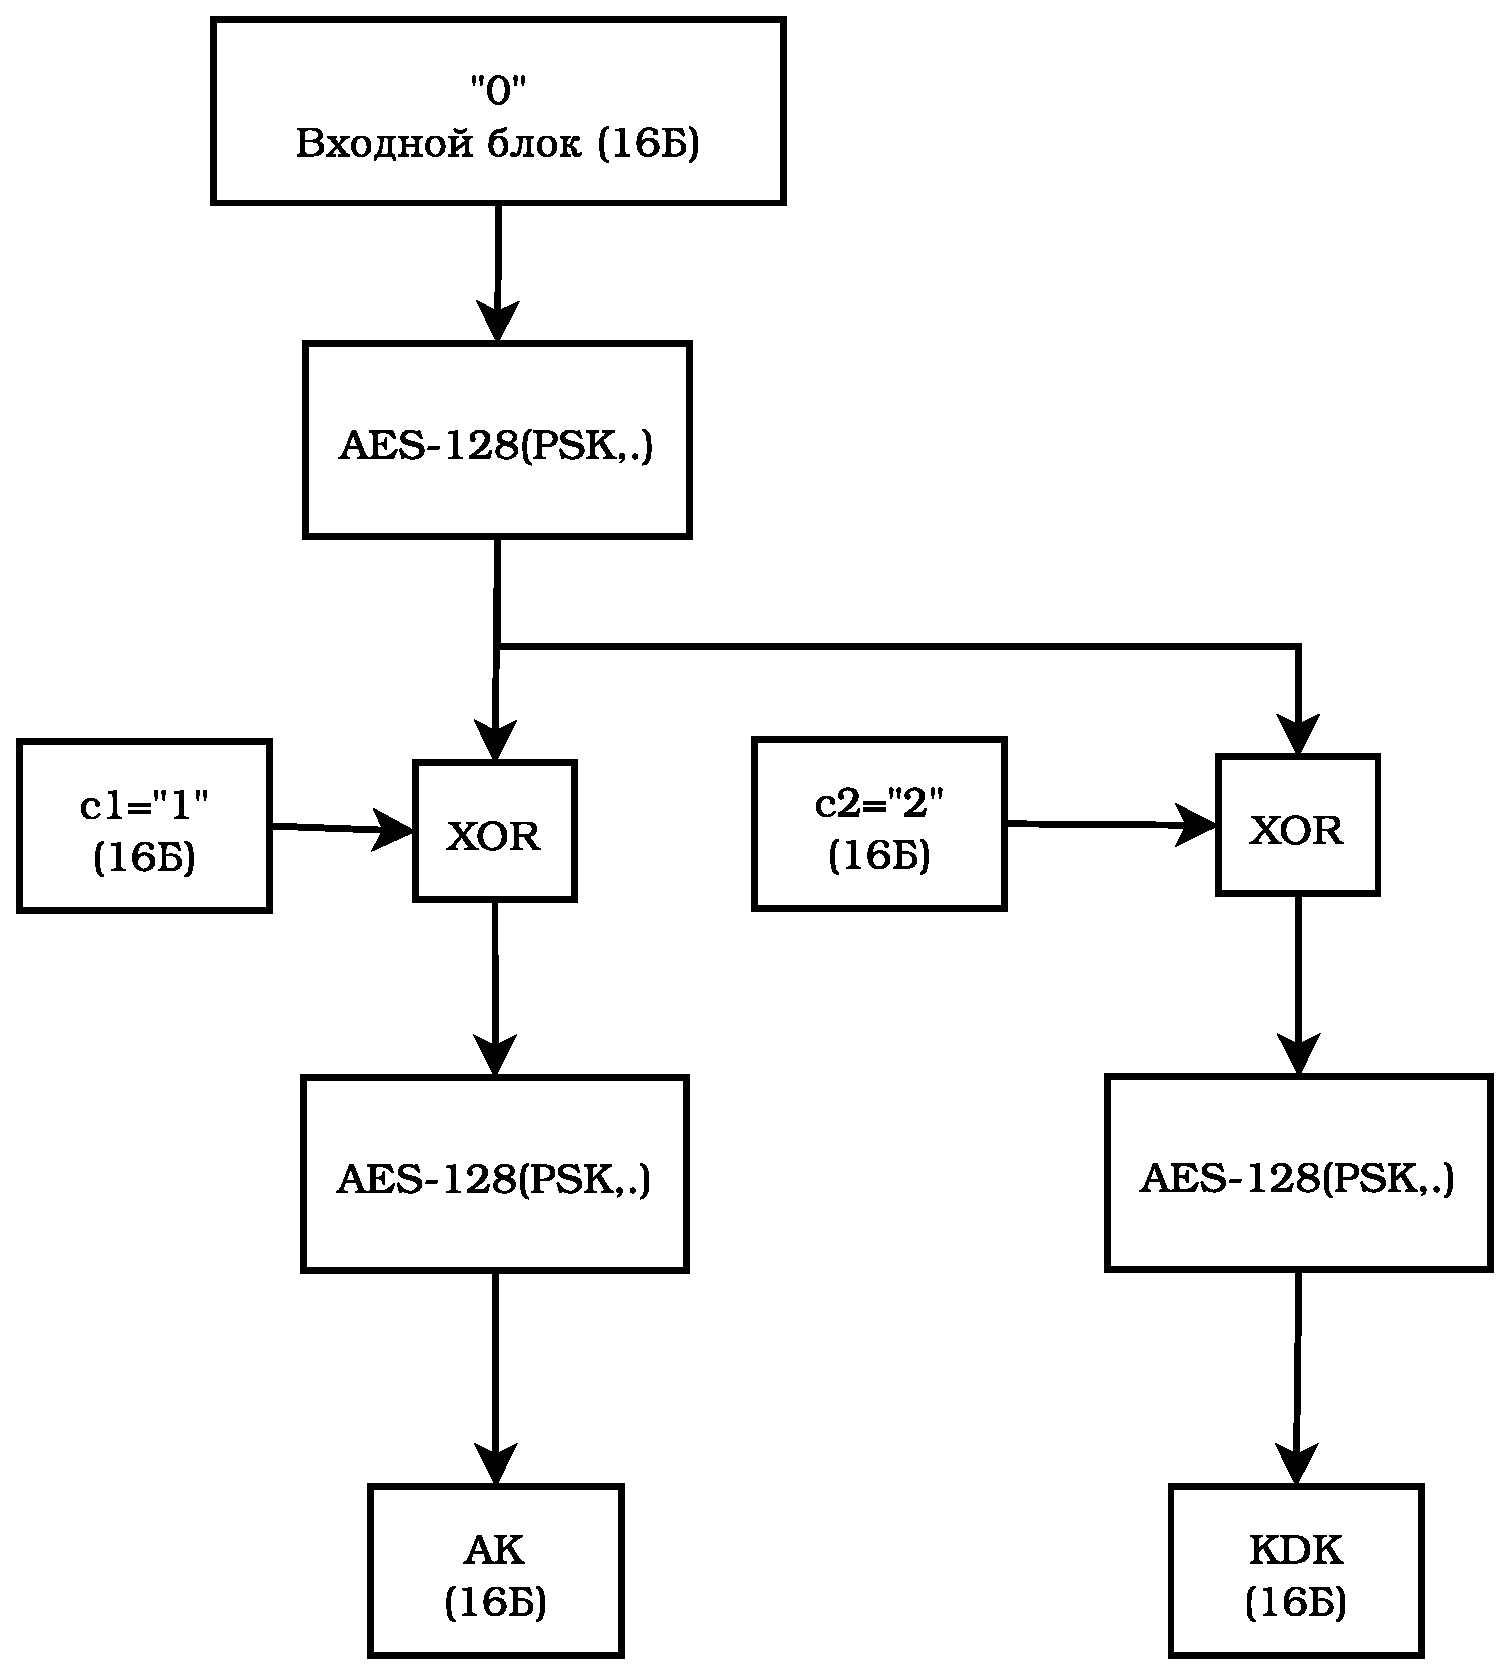
\includegraphics[width=0.9\linewidth]{./pictures/key_derivation}}
\caption{Генерация AK и KDK из PSK}
\label{img:key_derivation}
\end{figure}

Входным блок, для простоты, всегда является ``0''. Данное значение можно расчитывать в завиимости от Пира исервера (например XOR от значений из NAI), но это не дает значительного увеличения безопасности и значительно усложняет схему. Для работы может быть выбрана любая константа, это не влияет на свойства безопасности. Разработчики просто выбрали ``0''.

\subsection{Обмен ключами аутентификации}

В EAP-PSK для аутентификации используется алгоритм, схожий с AKEP2, который описан в документе ``Entity Authentication and Key Distribution'' (EAKD).

AKEP2 состоит из полутора раундов обмена, которые представлены на рисунке \ref{img:akep2}.

\begin{figure}[h!]
\center{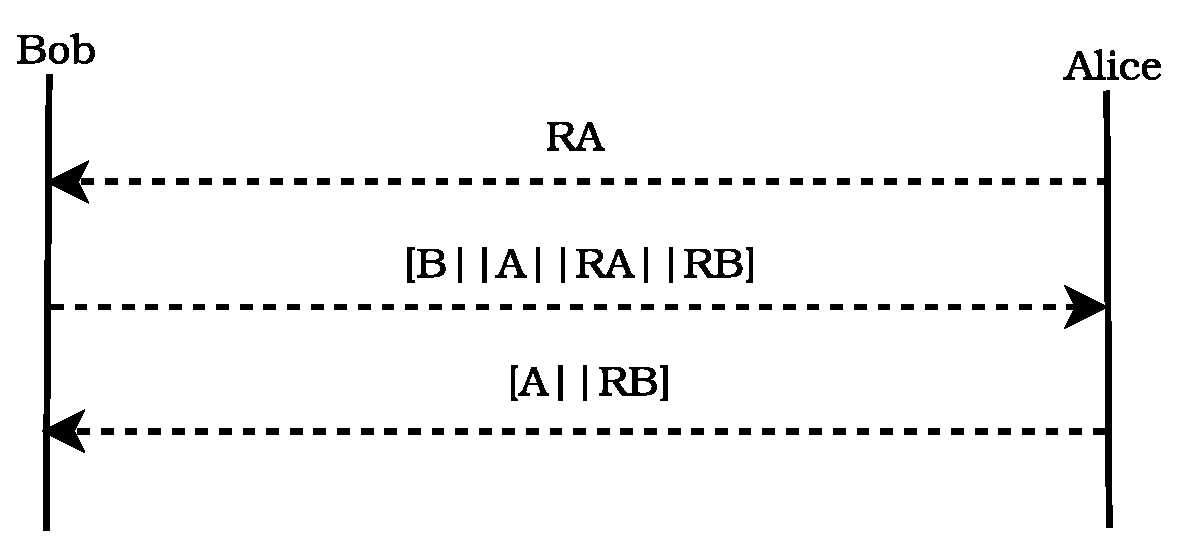
\includegraphics[width=0.9\linewidth]{./pictures/akep2}}
\caption{Описание AKEP2}
\label{img:akep2}
\end{figure}

Стоит отметить, что EAKD фокусируется на теоритической критпографии, а не на протоколах используемых в реальных условиях. Как описано в разделе ``Out-Of-Band-Data'' EAKD, Алиса отправляет A (её идентификатор) Бобу, затем Боб может выбрать соответствующие данные для продолжения обмена. Для EAP-PSK механизм изменен. AKEP2 для EAP-PSK представлен на рисунке \ref{img:eap-akep2}.

\begin{figure}[h!]
\center{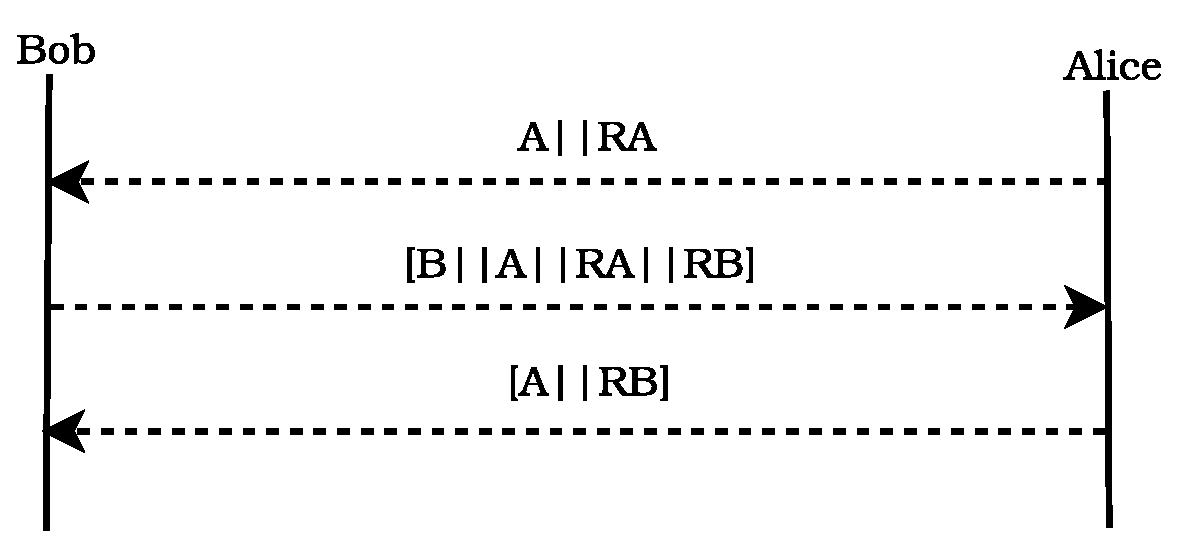
\includegraphics[width=0.9\linewidth]{./pictures/eap-akep2}}
\caption{Описание AKEP2 для EAP-PSK}
\label{img:eap-akep2}
\end{figure}

В AKEP2:

\begin{itemize}
\item RA и RB случайные числа, выбранные Алисой и Бобом соответственно;
\item A и B идентификаторы Алисы и Боба. Они помогают Алисе и Бобу выбрать ключи, которые они будут использовать при аутентификационном обмене друг с другом.
\item MACи (В разделе 1.3 есть описание оператора ``[]'') вычисляются с использованием заранее определенного ключа.
\end{itemize}

В EAP-PSK данный механизм реализован:

\begin{itemize}
\item Алиса выступает в роли сервера, а Боб в роли Пира;
\item RA и RB - 16-байтовые случайные числа. В нотации раздела 4.1: RA = RAND\_S, RB = RAND\_P;
\item A и B - NAI Алисы и Боба соответственно. В нотации раздела 4.1: A = ID\_S и B = ID\_P;
\item MAC - CMAC с использованием AES-128. Для подсчета MAC используется AK. MAC представляет собой 16-байтовую последовательность;
\item AES-128 в режиме счетчика использует KDK для генерации сессионного ключа. Сессионный ключ является результатом данного аутентификационного обмена.
\end{itemize}

CMAC был выбран в качестве алгоритма подсчета MAC, потмоу что он способен обрабатывать сообщения произвольной длины и ввиду его простой реализации. Данный алгоритм поддерживается в актуальном состоянии криптографическим сообществом. CMAC рекомендован NIST. CMAC детально описан в документе ``Recommendation for Block Cipher Modes of Operation: The CMAC Mode for Authentication''.

В AKEP2 обмен ключами является ``неявным'': Сессионные ключи получаются из RB. В EAP-PSK сессионные ключи выводяться из RAND\_P с использованием KDK и AES-128 в режиме счетчика, описанного в документе ``The Security of One-Block-to-Many Modes of Operation''. Данный режим был выбран поскольку это ростая схема генерации ключей, которая реализована на блочном шифре, так же эта схема имеет доказательство своей надежности. Режим счетчика является функцие, увеличивающей размер блока данных в t раз, где t >= 2. Генерация сессионных ключей представлена на рисунке \ref{img:sk_derivation}.

\begin{figure}[h!]
\center{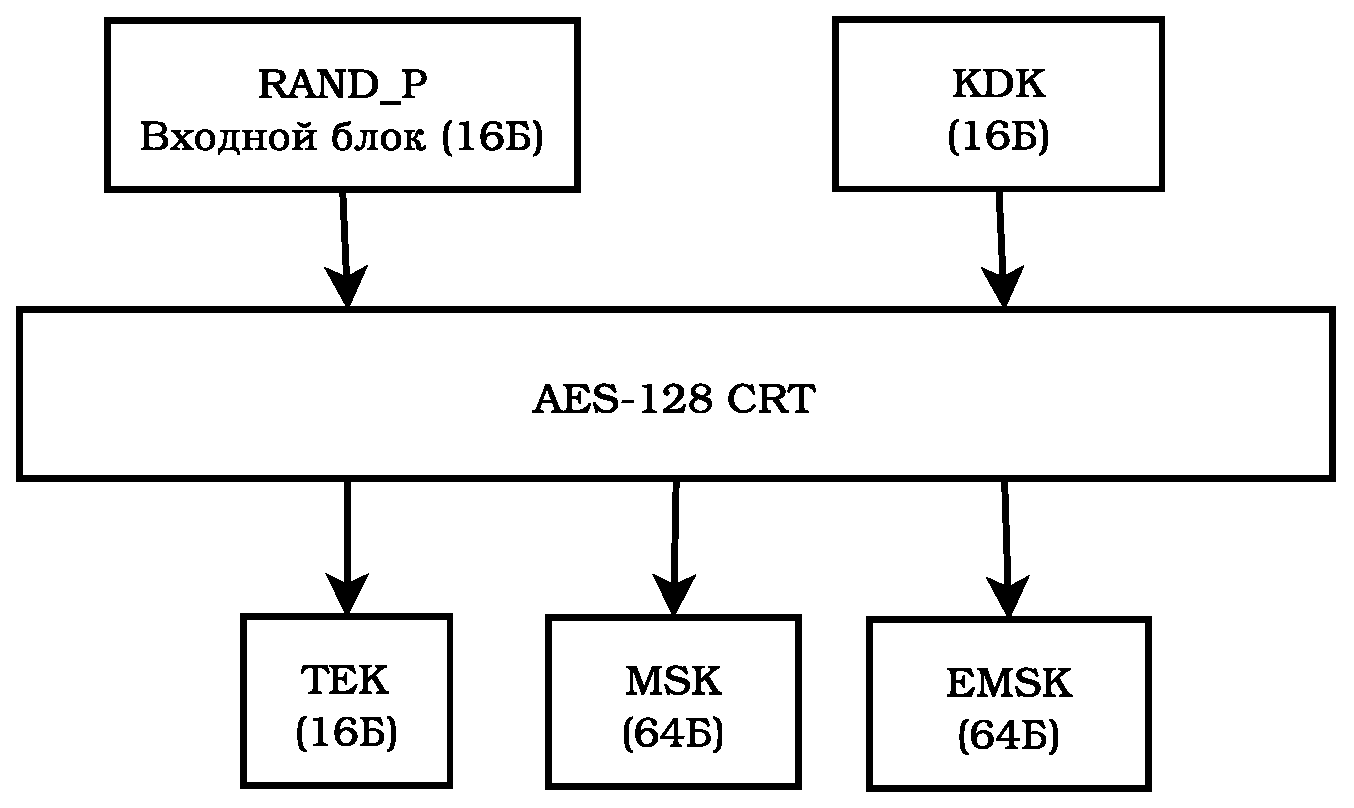
\includegraphics[width=0.9\linewidth]{./pictures/sk_derivation}}
\caption{Генерация сессионных ключей}
\label{img:sk_derivation}
\end{figure}

Входыми данными для генерации сессионных ключей служит RAND\_P.

На выходе генератора мы получаем сессионные ключи:

\begin{itemize}
\item 16-байтовый TEK (первый блок);
\item 64-байтовый MSK (конкатинация 2 - 5 блоков);
\item 64-байтовый EMSK (конкатинация 6 - 9 блоков).
\end{itemize}

Более детально алгоритм генерации сессионных ключей представлен на рисунке \ref{img:sk_derivation2}.

\begin{figure}[h!]
\center{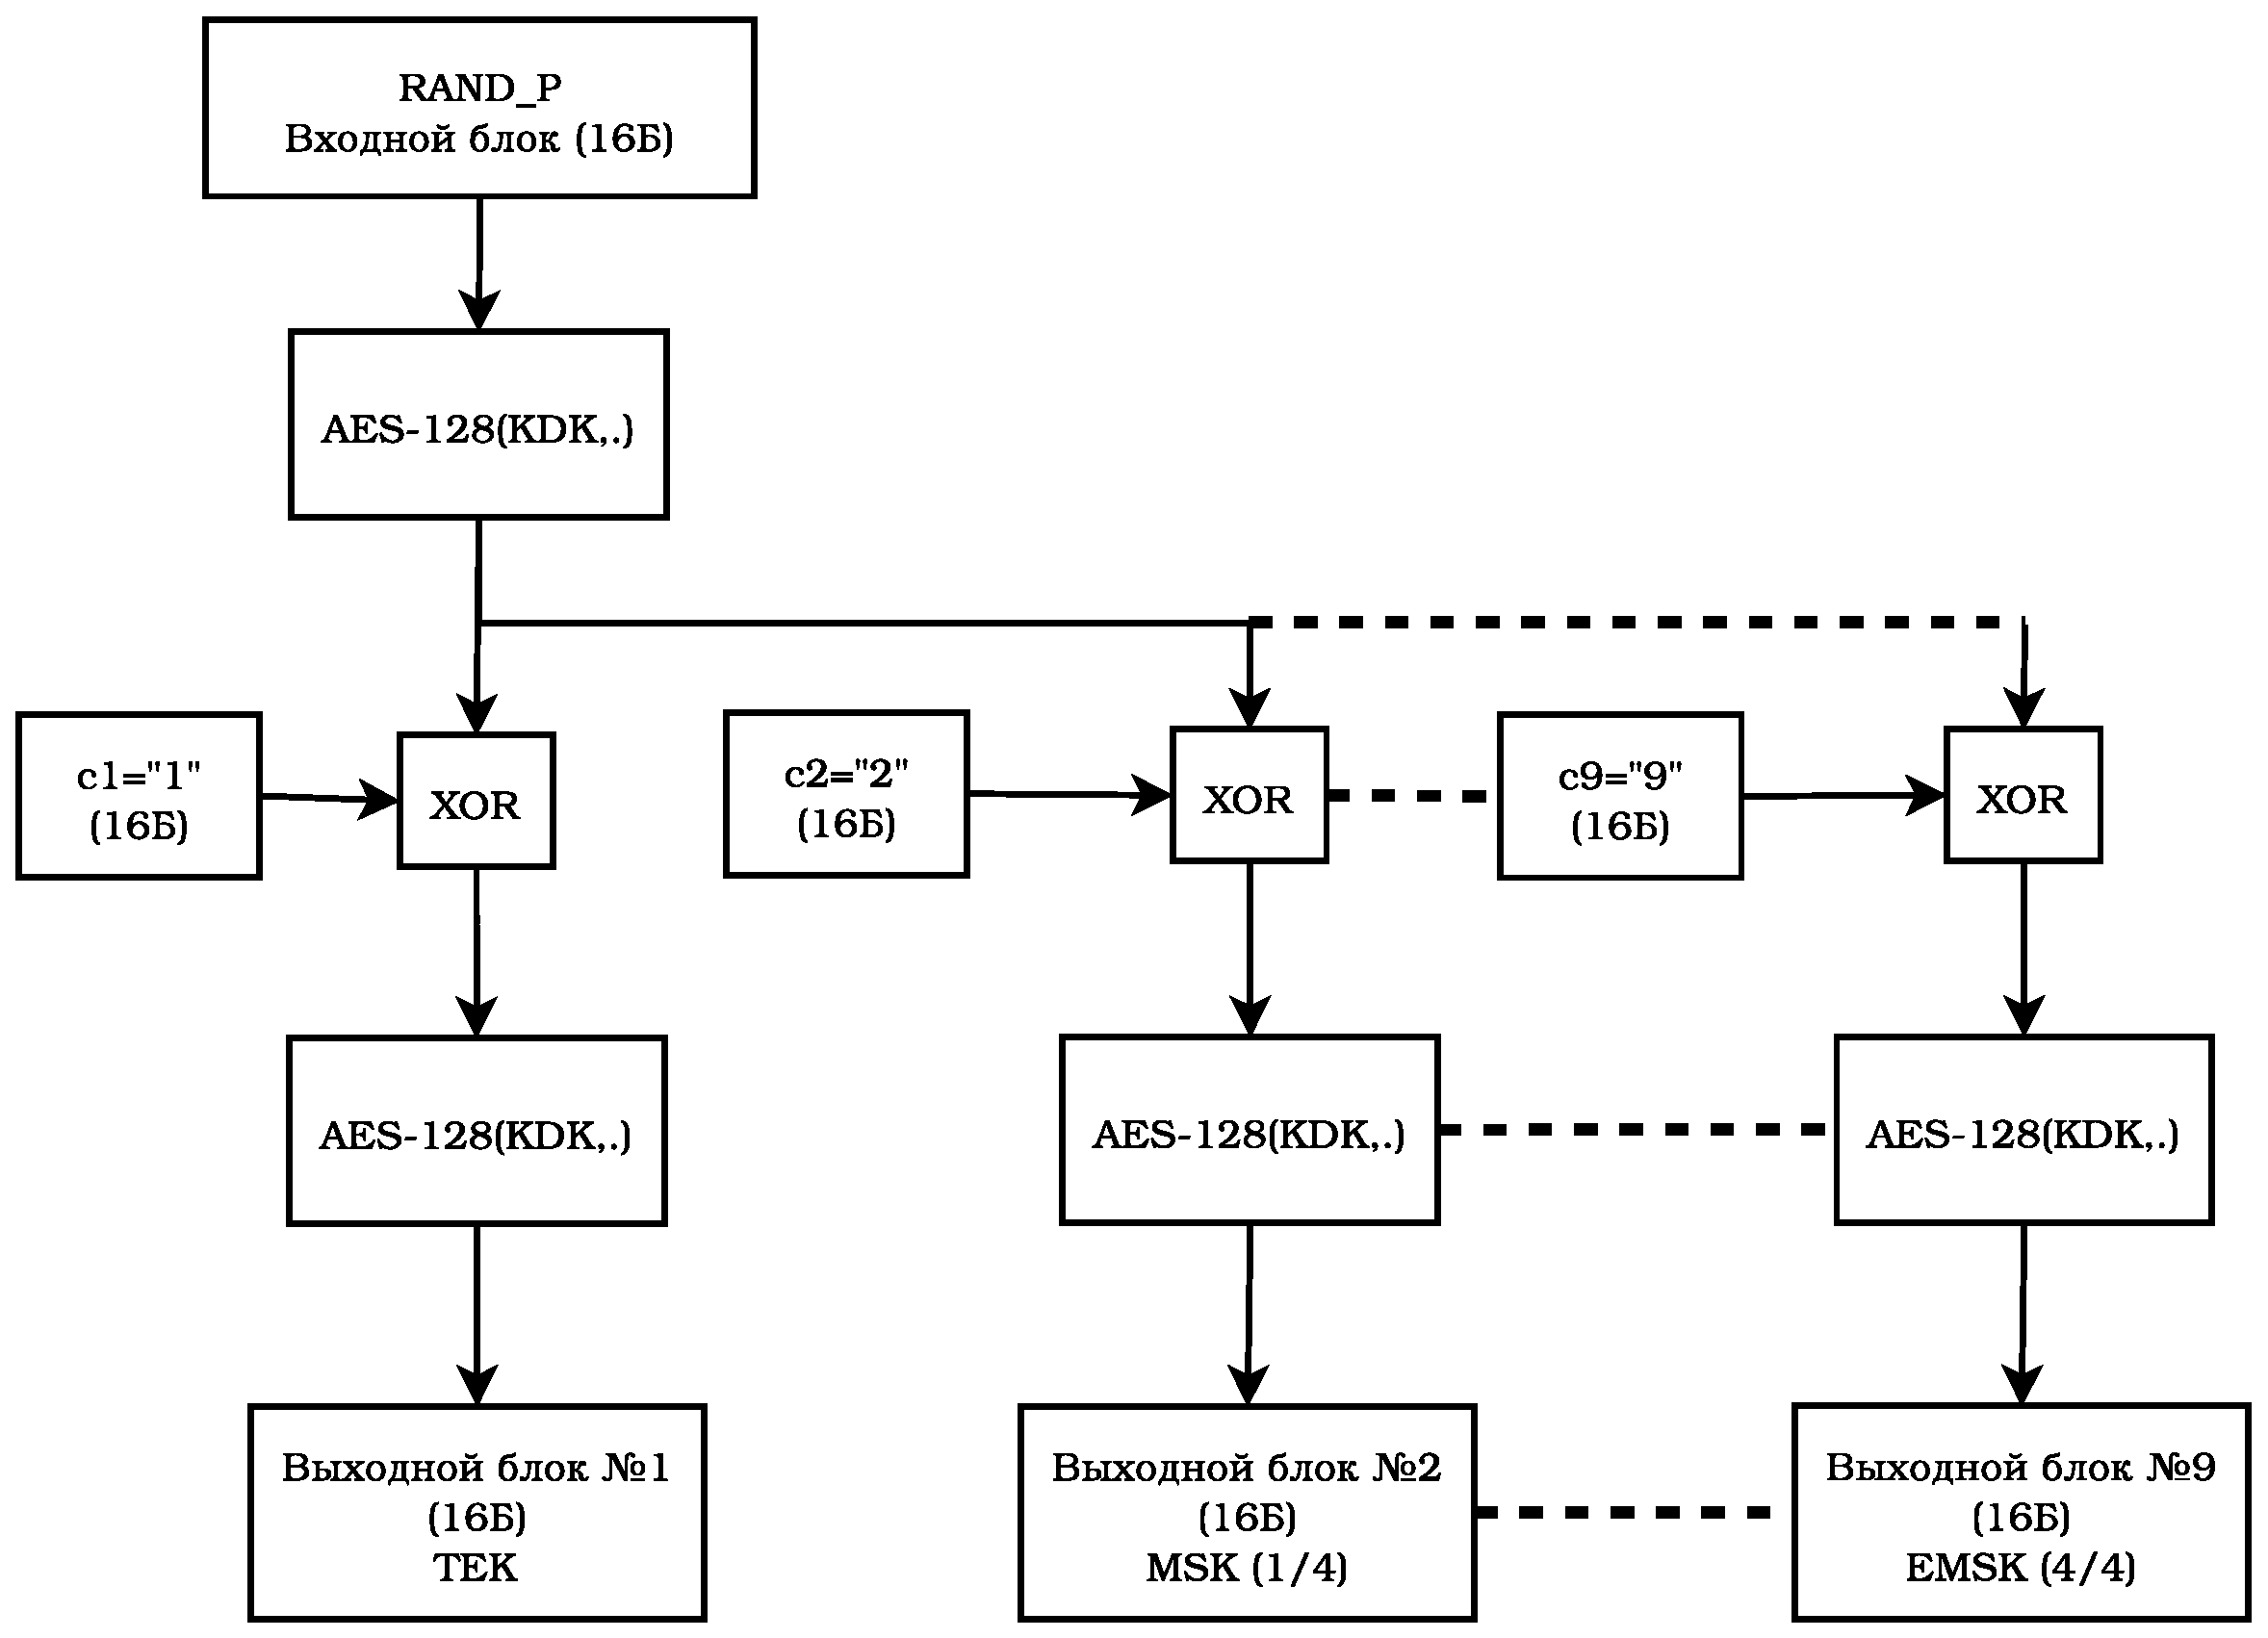
\includegraphics[width=0.9\linewidth]{./pictures/sk_derivation2}}
\caption{Генерация сессионных ключей}
\label{img:sk_derivation2}
\end{figure}

Значения счетчика соответствуеют первым t целым числам (тоесть ci = ``i'', где 1 <= t <= 9).

Ключивая информация является закрытой и должна обрабатываться соответствующим образом (подробности в разделе 8.10).

\subsection{Защищенный канал}

EAP-PSK предоставляет защищенный канал обмена данными для участников аутентификационного обмена в случае успешной аутентификации. В настоящее время этот канал используется для защищенного обмена результирующей индикации, но может быть использован расширениями протокола.

EAP-PSK использует режим работы EAX криптографического примитива для построения защищенного канала. Детальное описание EAX режима представлено в документе ``The EAX mode of operation''. На рисунке \ref{img:protected_channel} показано как используется EAX для построения защищенного канала в EAP-PSK.

\begin{figure}[h!]
\center{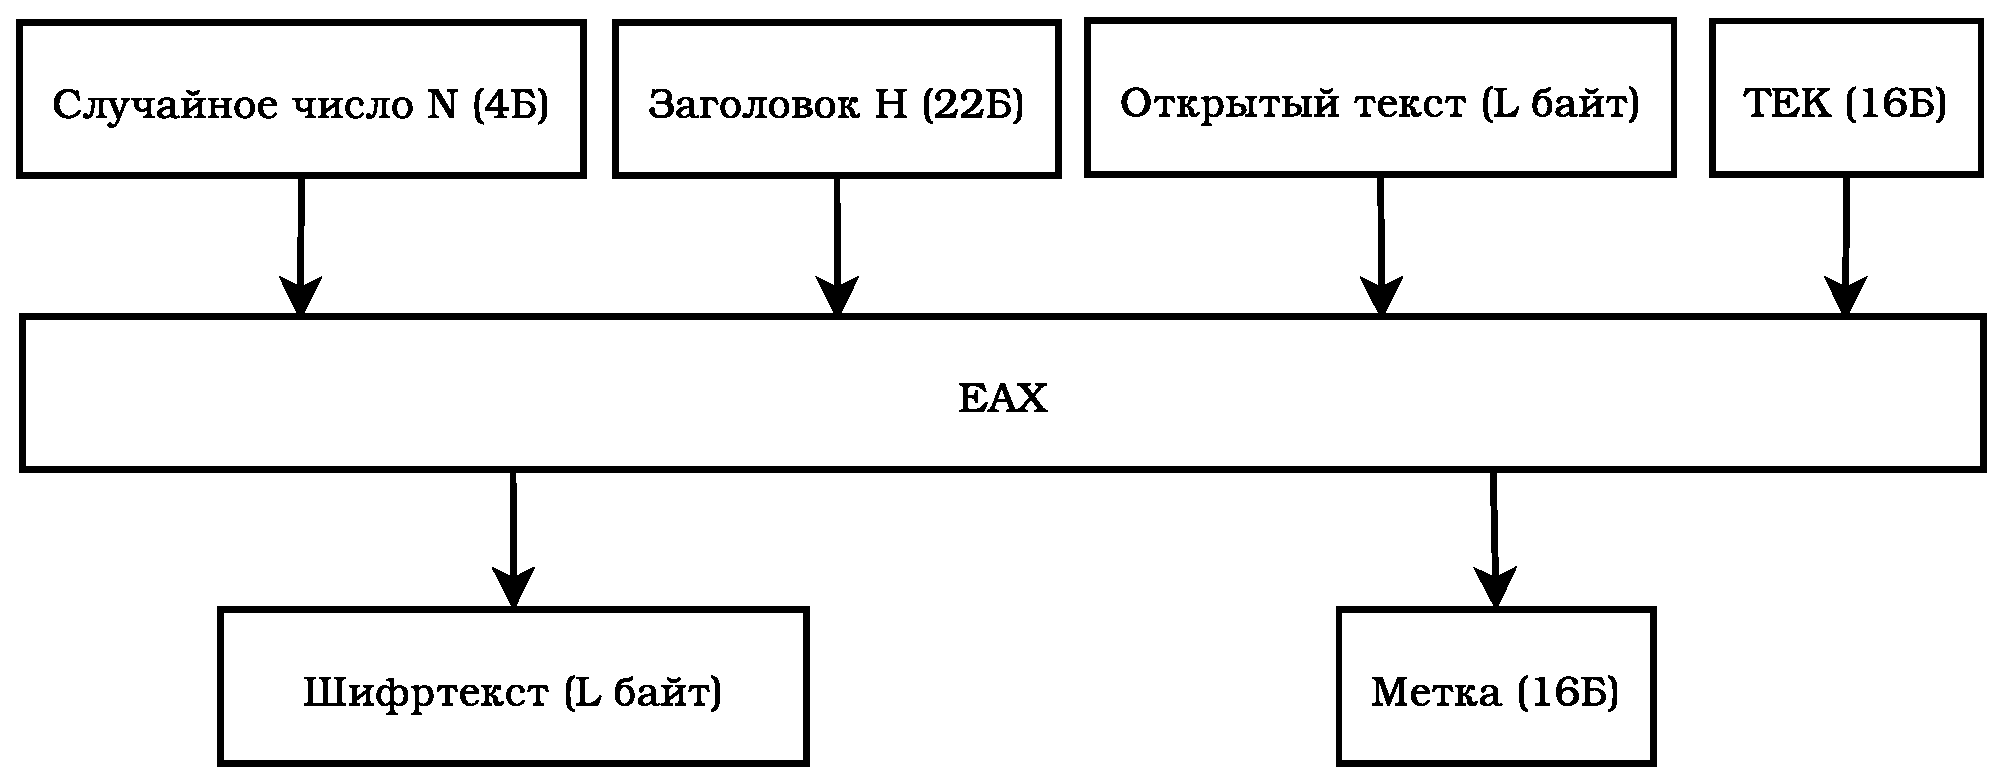
\includegraphics[width=0.9\linewidth]{./pictures/protected_channel}}
\caption{Защищенный канал}
\label{img:protected_channel}
\end{figure}

Защищенный канал:

\begin{itemize}
\item предоставляет защиту от повторений;
\item зашифровывает и аутентифицирует передаваемую информацию, которая становиться зашифрованной полезной нагрузкой. Зашифрованная полезная нагрузка не должна превышать 960 байт (пояснения в разделах 5.3, 5.4 и 8.11);
\item передает заголовок в открытом виде.
\end{itemize}

EAX основывается на алгоритме шифрования AES-128.

В качестве ключа в данном случае AES-128 испольузет TEK.

Случайное число N используется для предоставления криптографической защиты при шифровании, аутентификации данных, а так же при защите от повторов. На самом деле N это 4 байтовая последовательность чисел, начинающаяся с <0> и увеличивающаяся на единицу при отправке каждого нового пакета EAP-PSK в рамках одного обмена данных, за исключением повторной передачи сообщения.

Длина N в четыре байта была выбрана для того, что бы избежать 16-байтовой арифметики. Поскольку EAX использует 16-байтовые случайные числа, N дополняется 96 нулевыми битами в его старших разрядах.

Криптографические алгоритмы не позволяют циклически заменять N. Если случилось маловероятное событие, заключающееся в том, что сервер отправил сообщение с N = <2**32 - 2>, сервер больше не сможет отправлять сообщения по данному защищенному каналу, так как это приведет к повторному установлению N = 0. Обмен сообщениями завершается либо после того как от Пира был получен EAP-PSK ответ с N = <2**32 - 1> и сервер завершает обмен (обычно пакетом EAP-Success или -Failure), либо в случае если обмен сообщениями не завершен и должен быть прерван (новый EAP-PSK обмен может быть начат с новой попытки аутентификации). Таким образом, в рамках одного защищенного канала может быть передано только 2**32 сообщений (чего не должно произойти на практике, так как это более 4 миллиардов сообщений).

Заголовок H состоит из первых 22 байт EAP-Request или EAP-Responce (то есть полей EAP Code, идентификатор, длина и Тип с последующими полями EAP-PSK Flags и RAND\_S). Хотя может показаться необычным, что слой EAP-PSK защищает инфомрацию нижележащего слоя это оснано в рекомендаций EAP (RFC3748, раздел 7.5) и реализовано на практике IETF (``IP Authentication Header'').

Откртытй текст - это полезная нагрузка пакета, которая защищается посредством шифрования, так же осуществляется контроль целостности открытого текста. Зашифрованная полезная нагрузка -- результат зашифрования открытого текста.

Тэг представляет собой MAC, который защищает заголовок и открытый текст. Проверка Тэга должна осуществляться только после успешной проверки числа N с целью защиты от повторной обработки ``старого'' пакета. Если Тэг успешно проходит проверку, то происходит расшифровка и восстановление открытого текста. Если Тэг не проходит проверку, то расшировывания не происходит и в журнал заносится информация об ошибке MAC. Длина Тэга составляет 16 байт для EAX. Криптографическое сообщество считает такую длину целесообразной.

EAX был выбран в основном из-за:

\begin{itemize}
\item того, что его реализаци опирается на реализацию OMAC, а OMAC1, его аналог, уже используется в EAP-PSK в части аутентификации. (Пожалуйста помните что OMAC1 и CMAC являются аналогами);
\item простоты реализации;
\item гарантии его надежности;
\item обладания свободной лицензией.
\end{itemize}
